% !TEX encoding = UTF-8
% !TEX program = pdflatex
\documentclass[a4paper,11pt,twoside,openright]{book}
\usepackage[T1]{fontenc}            % imposta la codifica dei font
\usepackage[utf8]{inputenc}         % lettere accentate da tastiera
\usepackage[english,italian]{babel} % per scrivere in italiano
\usepackage{blindtext}              % genera testo fittizio
\usepackage{booktabs}               % gestisce al meglio la rappresentazione in tabelle
\usepackage[dvipsnames,usenames]{color}
\usepackage{comment}                % su puo' commentare un'intera porzione di testo
\usepackage{emptypage}              % per avere il layout vuoto di una pagina bianca
\usepackage{graphicx}               % per inserire immagini
\usepackage{ifthen}                 % permette di inserire anche il ciclo while
\usepackage{latexsym}               % permette di inserire i simboli di LaTeX
\usepackage{listings}               % per scrivere codice di programmazione
\usepackage{lipsum}                 % genera testo fittizio
\usepackage{quoting}                % rappresentare al meglio le citazioni
\usepackage{shorttoc}               % indice abbreviato
\usepackage{textcomp}               % collezione di simboli
\usepackage{verbatim}               % permette di inserire il testo cosi' come appare, senza interpretazione
\usepackage{url}                    % per scrivere gli indirizzi Internet
% \usepackage[section]{placeins}      % confina le immagini all'interno dei paragrafi in cui sono inserite (da usare solo se si hanno molte immagini con poco testo)

% controllo la sillabazione delle parole tra parentesi
% le parole tra parentesi NON saranno sillabate per andare a capo
% \hyphenation{VMWare VirtualBox Microsoft Windows Enterprise}

\pagestyle{headings}

\begin{document}
%%%%%%%%%%%%%%%%%%%%%%%%%%%%%%%%%%%%%%%%%%%%%%%%%%%%%%%%%%%%%%%%%%%%%%%%    
%    PARTE INTRODUTTIVA    %%%%%%%%%%%%%%%%%%%%%%%%%%%%%%%%%%%%%%%%%%%%%
%%%%%%%%%%%%%%%%%%%%%%%%%%%%%%%%%%%%%%%%%%%%%%%%%%%%%%%%%%%%%%%%%%%%%%%%    
  \frontmatter
  % scrive la copertina
  \thispagestyle{empty}
  \vrule
  \vbox{\vskip 1.0cm \vfil {\Large 
    % qui scrivere Cognome Nome allievo
    *** ***
    }\vfil\vbox{\vskip 4.5cm \vfil {\Huge \bfseries  
    % qui scrivere il titolo della guida
    Windows Server 2008
    \vfil}
    \LARGE \itshape \vskip 0.5cm {Installazione}
    {\vskip 0.5cm \itshape \LARGE 
    % qui scrivere l'eventuale sottotitolo
    %\vfil}{\vskip 3.5cm \itshape \normalsize 
    % note aggiuntive
    }\vfil\vbox{\vskip 5cm \vfil 
    
\includegraphics[scale=0.8]{images/irigem} \vfil 
    \makebox[3.3cm][s]{\Large 
    A.S. 2 0 1 8 / 1 9
    } \vfil
    }}
  }

  % scrive l'indice
  \tableofcontents

  \mainmatter

% v2.0 - 30.09.2018
%%%%%%%%%%%%%%%%%%%%%%%%%%%%%%%%%%%%%%%%%%%%%%%%%%%%%%%%%%%%%%%%%%%%%%%%    
%    PARTE PRINCIPALE    %%%%%%%%%%%%%%%%%%%%%%%%%%%%%%%%%%%%%%%%%%%%%%%
%%%%%%%%%%%%%%%%%%%%%%%%%%%%%%%%%%%%%%%%%%%%%%%%%%%%%%%%%%%%%%%%%%%%%%%%    

% Qui di seguito e' riportato un esempio di scrittura del codice da usare 
% per la creazione della tesina finale; per realizzare e consegnare una 
% sola guida bisogna mettere gli opprtuni commenti nelle righe che non 
% servono.

% Tutte le righe che iniziano col comando \part servono per creare le 
% varie SUDDIVISIONI PER OGNI MATERIA e lo si fa con la tesina finale,
% quindi se bisogna consegnare una guida sola, bisogna commentare tutte
% le righe che iniziano con \part aggiungendo ad inizio riga il simbolo 
% della percentuale, proprio come in queste righe.

% Tutte le righe che iniziano con \input servono per INCLUDERE tutte
% le guide che si desiderano e fare in modo che appaiano tutte insieme 
% in un unico documento.

% Il nome del file di ogni guida va creato a fianco e poi riportato
% all'interno del comando \input, cosi' come specificato negli esempi
% che seguono.

% Qui di seguito c'e' un esempio di creazione di una tesina di fine anno 
% con quattro divisioni per quattro materie, ognuna delle quali specificata 
% dalla riga col comando \part 
% Per ogni materia sono state specificate tutte le guide da includere.

% Per personalizzare il tutto basta modificare e/o aggiungere le varie
% sezioni delle varie materie e includere le guide desiderate, commentando
% le righe che non servono.
% Per una migliore gestione delle guide da aggiungere, si consiglia
% quanto segue:
% - ogni volta che durante l'anno bisogna creare una guida, basta commentare
%   tutte le righe che non servono e lasciare solo quella che inizia con 
%   \input e specifica il nome della guida da realizzare
% - far iniziare il nome della guida con il nome della materia e proseguire
%   con l'argomento trattato all'interno della guida stessa, cosi' come 
%   negli esempi
% - creare all'interno della cartella images, specificata a fianco, una 
%   cartella con lo stesso nome della guida che si vuole aggiungere e
%   aggiungere li' dentro tutte le immagini relative alla guida specificata
% - a fine anno, per creare la tesina, basta togliere i commenti dalle righe
%   di tutte le materie e da tutte le guide da includere

\begin{document}
\chapter{Installazione}
Si vuole illustrare come installare il sistema operativo Windows Server 2008.
Tale procedura può essere eseguita sia in ambiente fisico, sia in ambiente virtuale
tramite l’uso dei più diffusi software di virtualizzazione come VMWare
o VirtualBox. In quest’ultimo caso si consiglia di utilizzare l’ultima versione
aggiornata del software di virtualizzazione per massimizzare la compatibilità
con il sistema operativo da installare.\\ \indent
I passi che saranno seguiti per portare a termine l’esperienza suddetta,
sono i seguenti:

\begin{itemize}
\item verifica dei requisiti hardware minimi
\item installazione
\item configurazione minimale
\end{itemize}

\section{Requisiti hardware}
Dal sito web di Microsoft [1] si nota come i requisiti minimi per l’installazione
di Windows Server 2008 siano i seguenti:
\\ {\scshape \bfseries Processore} : 1 GHz (per cpu x86) o 1.4 GHz (per cpu x64)
\\ {\scshape \bfseries Memoria} : 512 MB
\\ {\scshape \bfseries Disco} : 10 GB
\\ {\scshape \bfseries Unità aggiuntive} : lettore DVD-ROM
\\ {\scshape \bfseries Video e periferiche} : monitor Super VGA (800 x 600), tastiera e mouse
\\ Questi requisiti sono da considerare solo per eseguire un’installazione di prova,
ma devono essere opportunamente ridimensionati nel caso in cui si voglia
realizzare un ambiente di produzione con vari servizi attivi come { \itshape file server,
active directory, application server, virtual cloud, } ecc

\section{Installazione}
Se si volesse valutare il sistema operativo prima di acquistarlo, è possibile
scaricare una copia di valutazione di 180 giorni dal sito web di Microsoft [2].
Dopo aver inserito il DVD nel lettore ed avviato il computer in modo che
esegua il boot dal dispositivo ottico, saranno chieste informazioni sulla lingua
(solo inglese, non si può cambiare), sul fuso orario (scegliere Italian) e sul
tipo di tastiera (scegliere Italian) (v. fig. \ref{fig:grab0003}).
\begin{figure}[htbp]
 \centering
 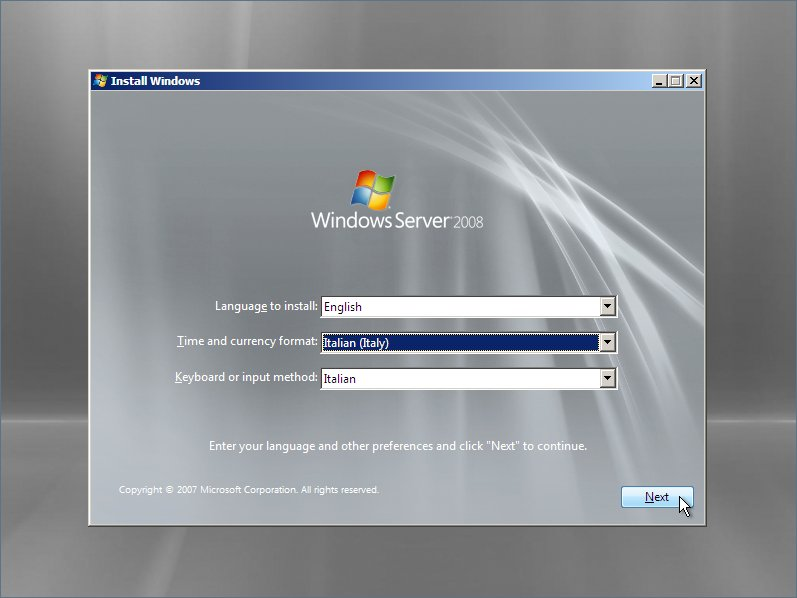
\includegraphics[scale=0.5]{images/grab0003}
 \caption{Richiesta della lingua, del fuso orario e del tipo di tastiera.}
\label{fig:grab0003}
\end{figure}

\indent Al passo successivo (fig. \ref{fig:grab0004}) selezionare Install now per proseguire con
l’installazione. Se invece fosse necessario ripristinare una precedente installazione
del sistema operativo da un backup fatto in precedenza, eseguire il
test della memoria o accedere al prompt dei comandi, allora potrebbe essere
utile selezioanre il collegamento Repair your computer, dove sono messi a
disposizione utili strumenti di ripristino e diagnostica.
\\ \indent A questo punto si richiede di inserire il codice della licenza (fig. \ref{fig:grab0005}), senza
il quale il periodo di valutazione sarebbe limitato a 60 giorni (estendibile a
240 [3]). Per motivi di praticità, in questa guida si è scelto di non inserire il
codice di licenza e di proseguire ugualmente (fig. \ref{fig:grab0006}).
\\ \indent Se non si inserisce il codice della licenza, sarà chiesta la versione del
sistema operativo da installare (fig. \ref{fig:grab0007}). Da notare che scegliendo Core Installation
si installerà il sistema operativo senza interfaccia grafica, lasciando
disponibile solo un ambiente a riga di comando.

\begin{figure}[htbp]
 \centering
 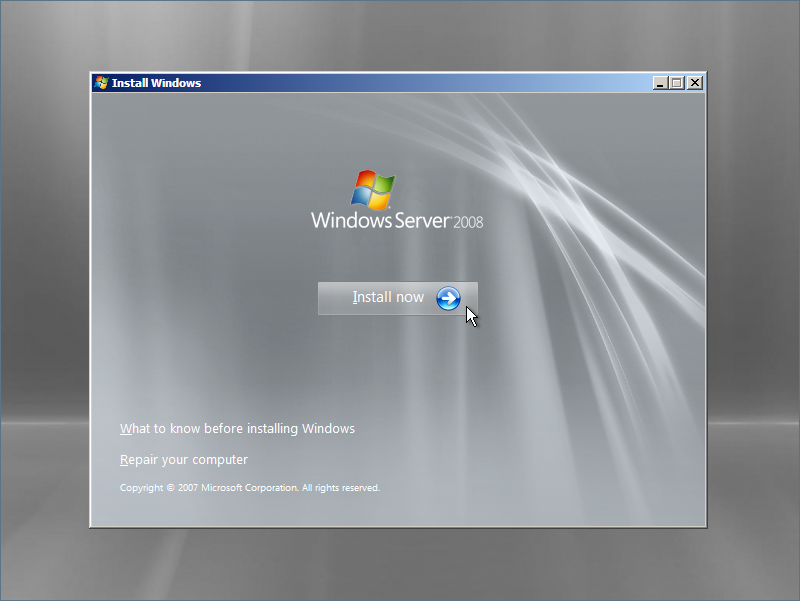
\includegraphics[scale=0.5]{images/grab0004}
 \caption{Selezionare Install now per proseguire.}
\label{fig:grab0004}
\end{figure}

\begin{figure}[htbp]
 \centering
 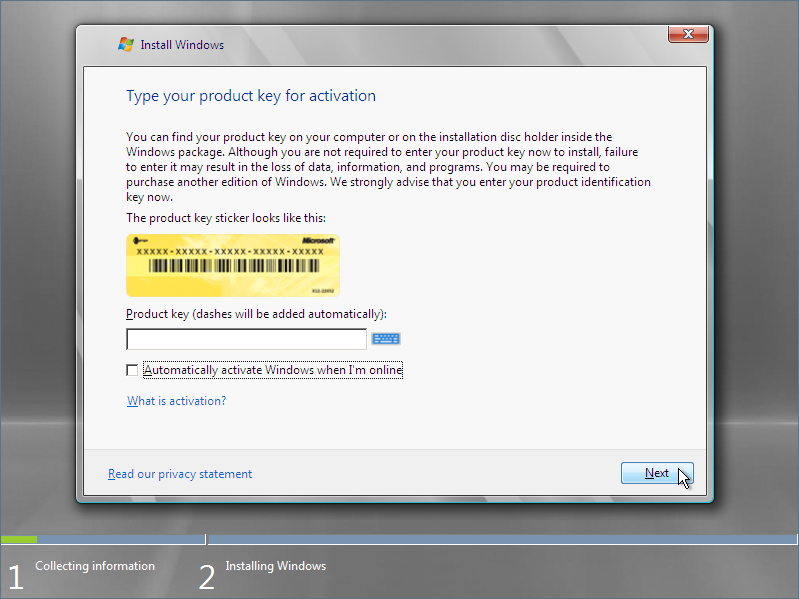
\includegraphics[scale=0.5]{images/grab0005}
 \caption{Inserire il numero di licenza.}
\label{fig:grab0005}
\end{figure}

\begin{figure}[htbp]
 \centering
 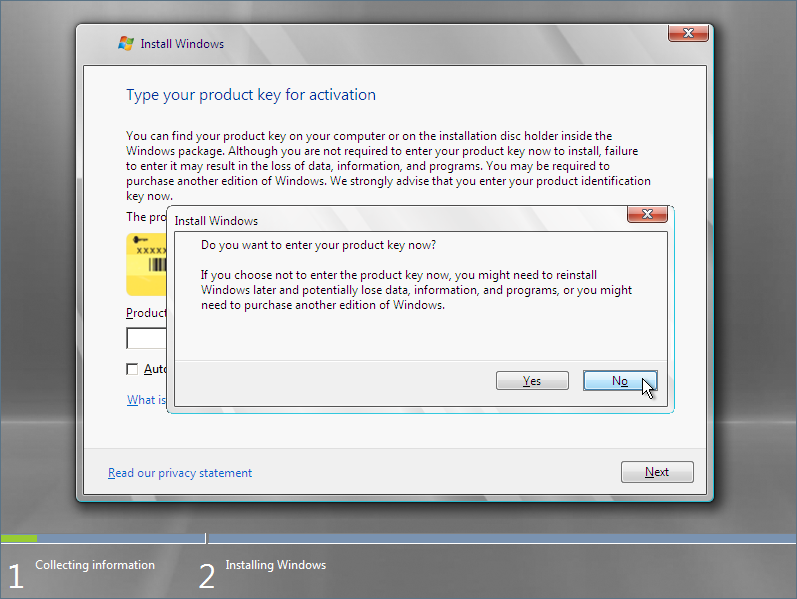
\includegraphics[scale=0.5]{images/grab0006}
 \caption{ Si può procedere anche senza inserire il numero di licenza.}
\label{fig:grab0006}
\end{figure}

\begin{figure}[htbp]
 \centering
 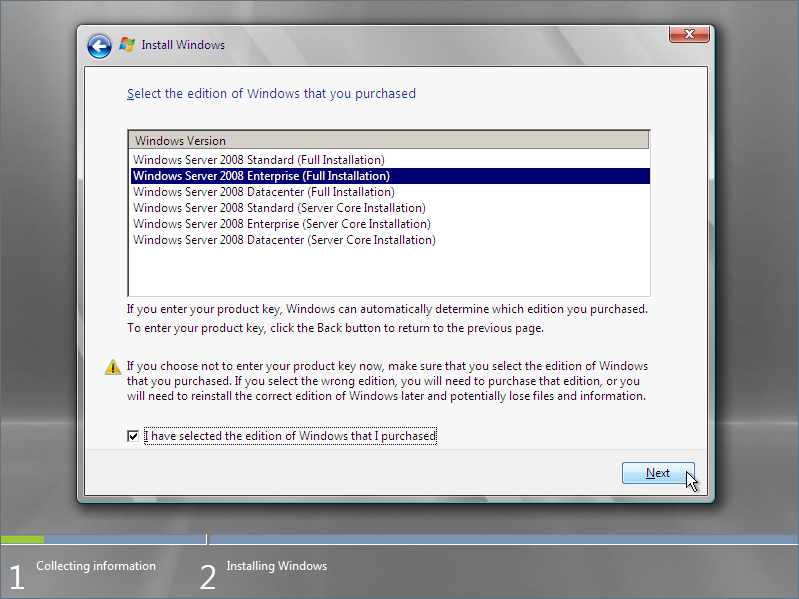
\includegraphics[scale=0.5]{images/grab0007}
 \caption{Scegliere la versione desiderata del sistema operativo.}
\label{fig:grab0007}
\end{figure}

\indent \newpage Nei tre passi successivi è richiesto di accettare la licenza sul software
(fig. \ref{fig:grab0008}), di selezionare l’operazione di installazione (fig. \ref{fig:grab0009}) e di scegliere il
disco in cui installare Windows (fig. \ref{fig:grab0010}).

\begin{figure}[htbp]
 \centering
 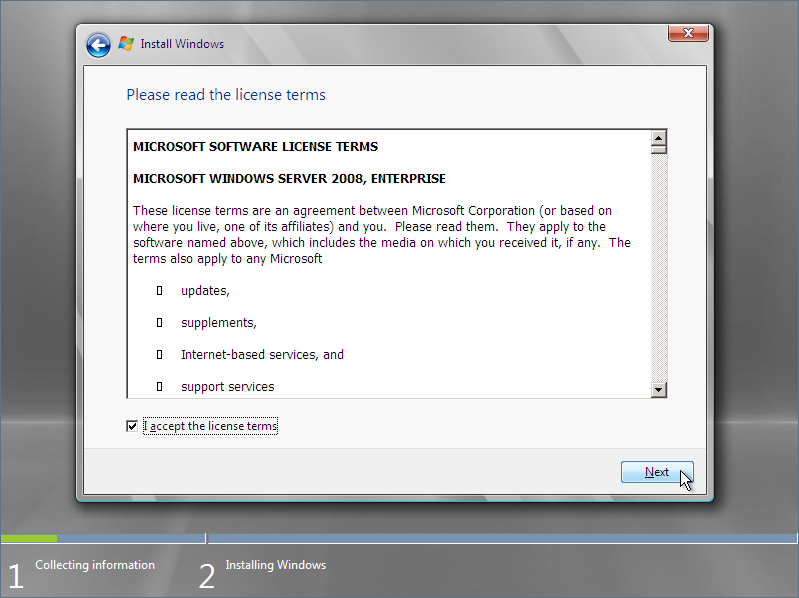
\includegraphics[scale=0.5]{images/grab0008}
 \caption{Leggere e accettare la licenza sul software.}
\label{fig:grab0008}
\end{figure}

\indent Al termine del processo di installazione (fig. \ref{fig:grab0011}), si presenta la schermata
di accesso con la richiesta di cambiare la password all’utente amministratore
(fig. \ref{fig:grab0012}). Nella scelta della nuova password, si raccomanda di utilizzare
una parola di almeno 8 caratteri contenente minuscole, maiuscole e numeri
(fig. \ref{fig:grab0013}). \\
\\ \indent Una volta assegnata la password (fig. \ref{fig:grab0014}), il sistema procederà con l’avvio
della sessione di accesso mostrando subito una schermata che propone
dei passi di configurazione del server, sia preliminari, sia avanzati (fig. \ref{fig:grab0015}).
Se la si chiude, viene subito proposta la schermata per la configurazione specifica
del server, che riprende un po’ alcune voci precedenti ma ne aggiunge
anche delle altre (fig. \ref{fig:grab0016}). \\
\\ \indent Se si chiude anche questa finestra, rimane finalmente visibile il desktop di
Windows (fig. \ref{fig:grab0017}). Successivamente saranno elencate alcune configurazioni
nel caso si voglia usare Windows Server quasi come fosse una workstation,
disabilitando ad esempio alcune caratteristiche proprie della versione Server
(CTRL+ALT+CANC al login, registratore eventi allo spegnimento, ecc.)

\begin{figure}[htbp]
 \centering
 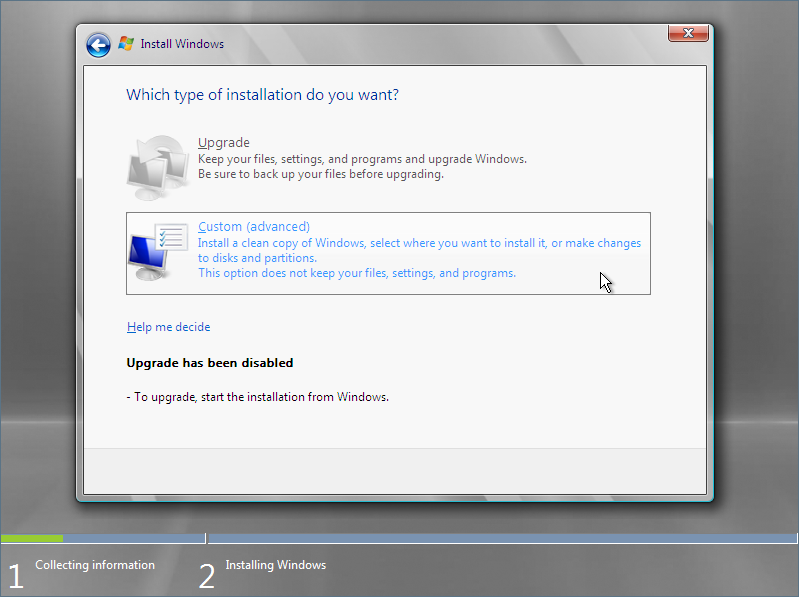
\includegraphics[scale=0.5]{images/grab0009}
 \caption{Selezionare l’operazione di installazione.}
\label{fig:grab0009}
\end{figure}

\begin{figure}[htbp]
 \centering
 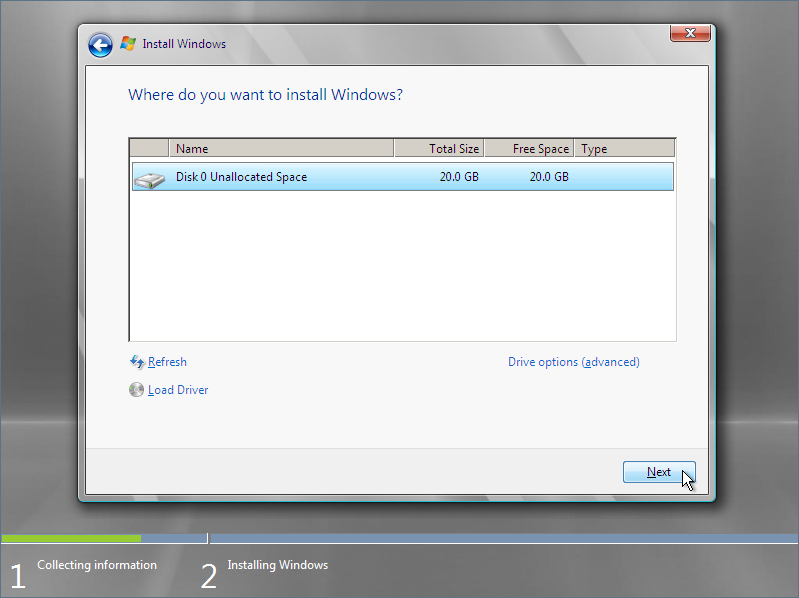
\includegraphics[scale=0.5]{images/grab0010}
 \caption{Scegliere il disco dove installare il sistema operativo.}
\label{fig:grab0010}
\end{figure}

\begin{figure}[htbp]
 \centering
 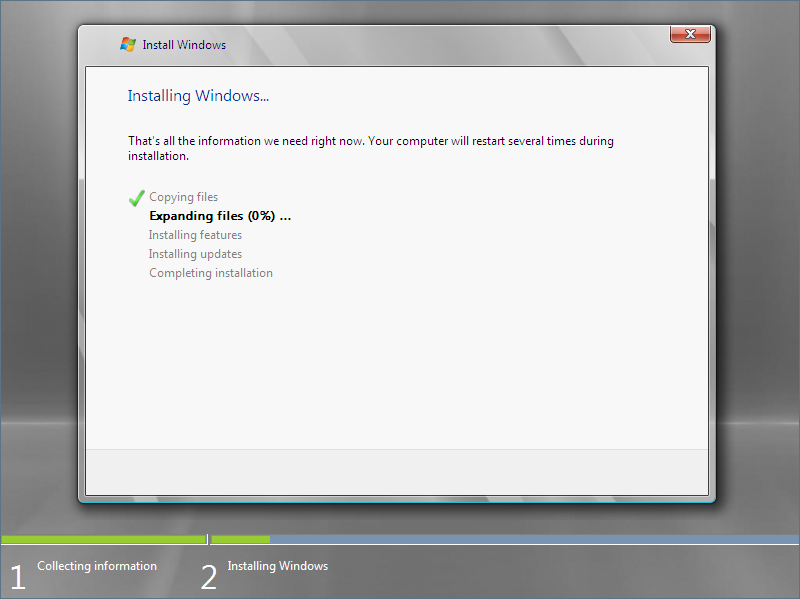
\includegraphics[scale=0.5]{images/grab0011}
 \caption{Processo d’installazione avviato.}
\label{fig:grab0011}
\end{figure}

\begin{figure}[htbp]
 \centering
 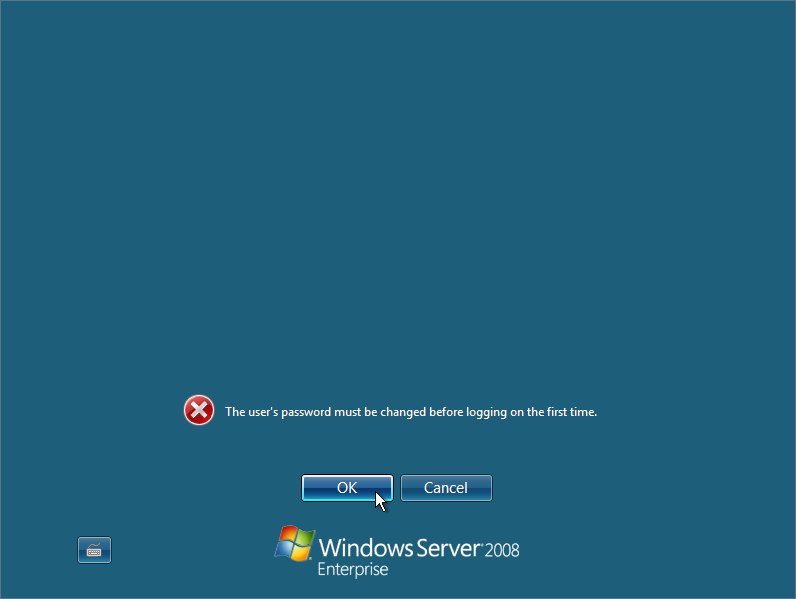
\includegraphics[scale=0.5]{images/grab0012}
 \caption{Avviso di cambio password per il primo utente (Administrator).}
\label{fig:grab0012}
\end{figure}

\begin{figure}[htbp]
 \centering
 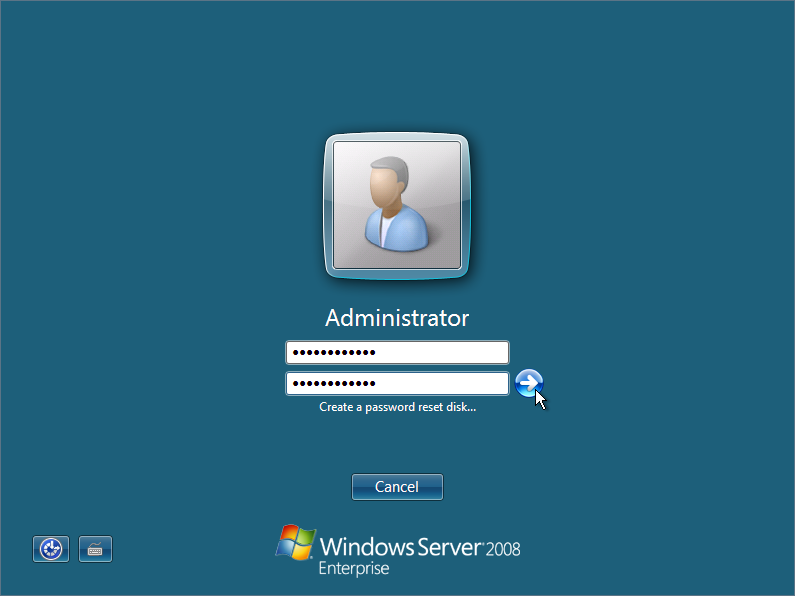
\includegraphics[scale=0.5]{images/grab0013}
 \caption{ Minimo 8 caratteri con minuscole, maiuscole e numeri.}
\label{fig:grab0013}
\end{figure}

\begin{figure}[htbp]
 \centering
 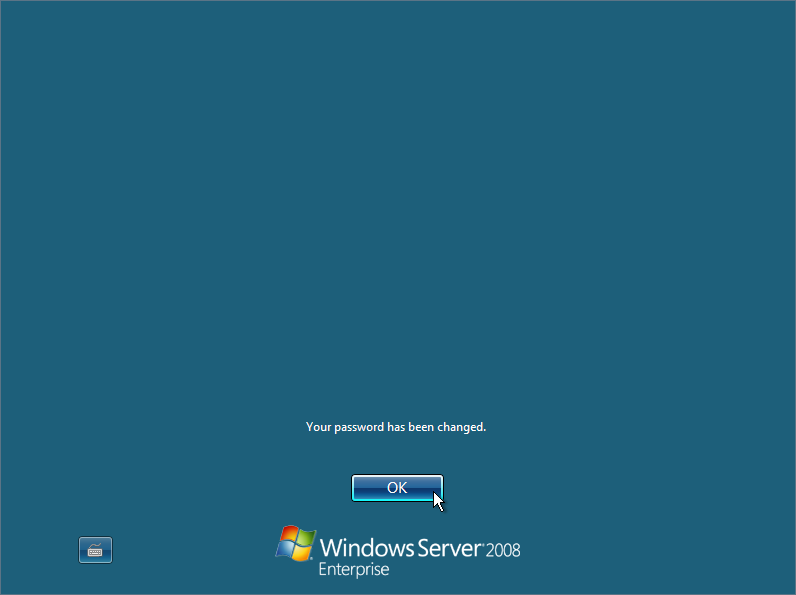
\includegraphics[scale=0.5]{images/grab0014}
 \caption{Se la scelta è corretta, l’accesso è garantito.}
\label{fig:grab0014}
\end{figure}

\begin{figure}[htbp]
 \centering
 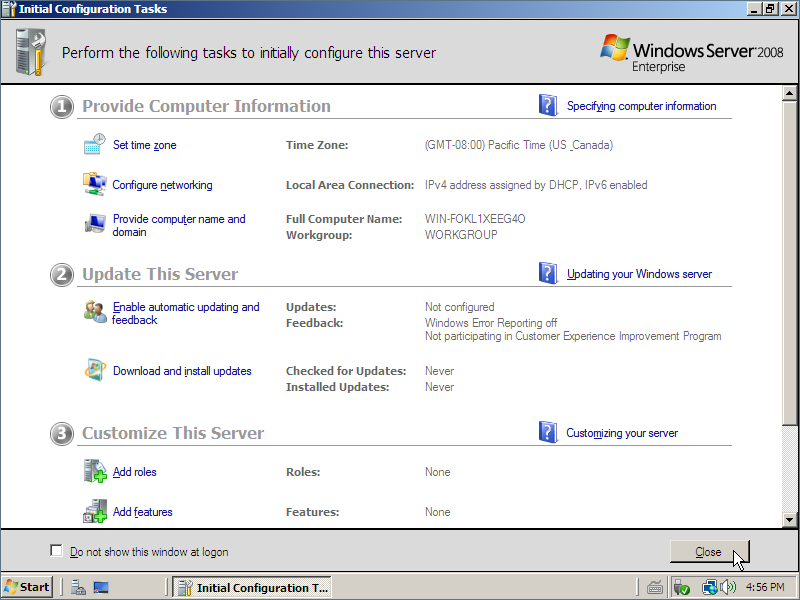
\includegraphics[scale=0.5]{images/grab0015}
 \caption{Fasi di configurazione proposte.}
\label{fig:grab0015}
\end{figure}

\begin{figure}[htbp]
 \centering
 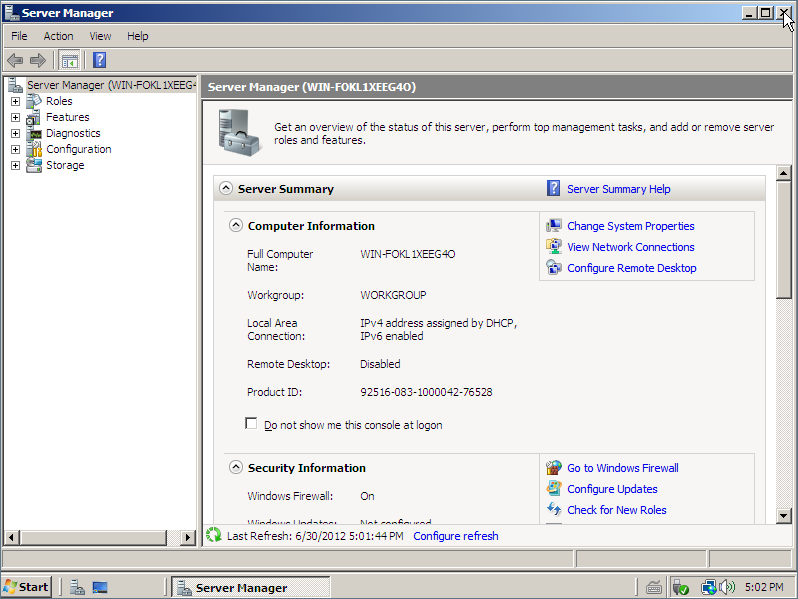
\includegraphics[scale=0.5]{images/grab0016}
 \caption{Utile finestra per la configurazione del server.}
\label{fig:grab0016}
\end{figure}

\begin{figure}[htbp]
 \centering
 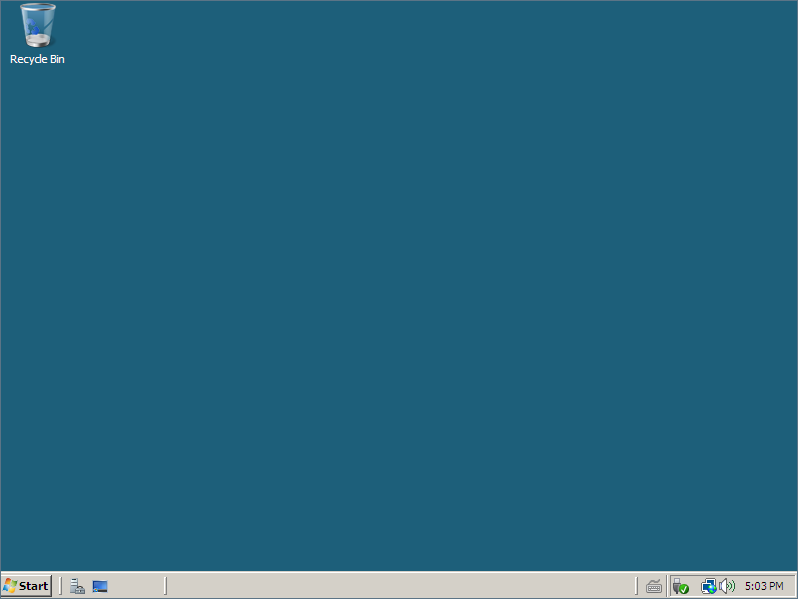
\includegraphics[scale=0.5]{images/grab0017}
 \caption{Il desktop.}
\label{fig:grab0017}
\end{figure}

\section{Shutdown Event Tracker}

Nel caso si sia in un ambiente di test e si desideri usare Windows Server con
alcuni accorgimenti che ne migliorino l’usabilità, sarà il caso di procedere
con alcune modifiche illustrate qui di seguito. Se si prova ad avviare il
processo di spegnimento, appare la finestra per la registrazione degli eventi
(fig. \ref{fig:grab0018}), proprio come nella precedente versione del sistema operativo. Per
disabilitare il registratore eventi durante le fasi di riavvio o spegnimento del
sistema, procedere come segue:

\begin{itemize}
    \item andare nel menù Start » Run e digitare gpedit.msc premendo poi OK.
A questo punto dovrebbe aprirsi la finestra Local Group Policy Editor.
    \item seguire il percorso Computer Configuration » Administrative Templates
e fare click su System.
    \item nell’elenco che appare, fare doppio click su Display Shutdown Event
Tracker, selezionare Disabled e poi premere OK per salvare (fig. \ref{fig:grab0024}).
\end{itemize}


\section{CTRL+ALT+DEL prompt}
Solitamente nelle versioni Server dei sistemi operativi Microsoft, viene richiesta
la pressione della combinazione di tasti CTRL+ALT+CANC prima di

\begin{figure}[htbp]
 \centering
 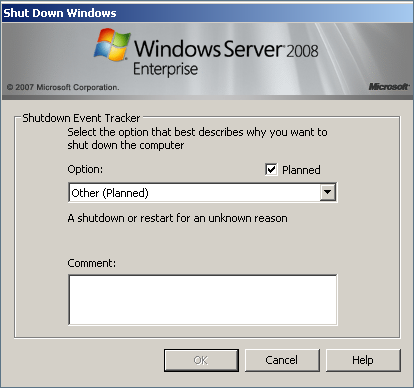
\includegraphics[scale=0.5]{images/grab0018}
 \caption{Il logger per le operazioni di spegnimento e riavvio.}
\label{fig:grab0018}
\end{figure}

\begin{figure}[htbp]
 \centering
 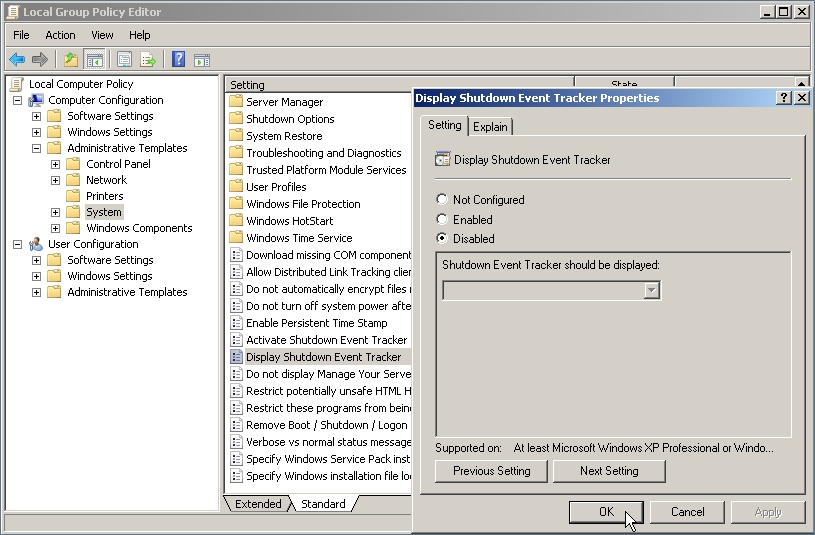
\includegraphics[scale=0.5]{images/grab0024}
 \caption{: Local Group Policy Editor.}
\label{fig:grab0024}
\end{figure}

poter eseguire il login. In situazioni di test in cui i riavvii possono essere frequenti,
potrebbe essere più comodo disabilitare questa richiesta. Procedere
come segue:

\begin{itemize}
    \item scegliere nel menù Start » Administrative Tools » Local Security Policy.
    \item seguire il percorso Local Policies » Security Options e fare doppio click
su Interactive logon: Do not require CTRL+ALT+CANC
    \item selezionare Enabled e poi premere OK per salvare (fig. \ref{fig:grab0025}).
\end{itemize}

\begin{figure}[htbp]
 \centering
 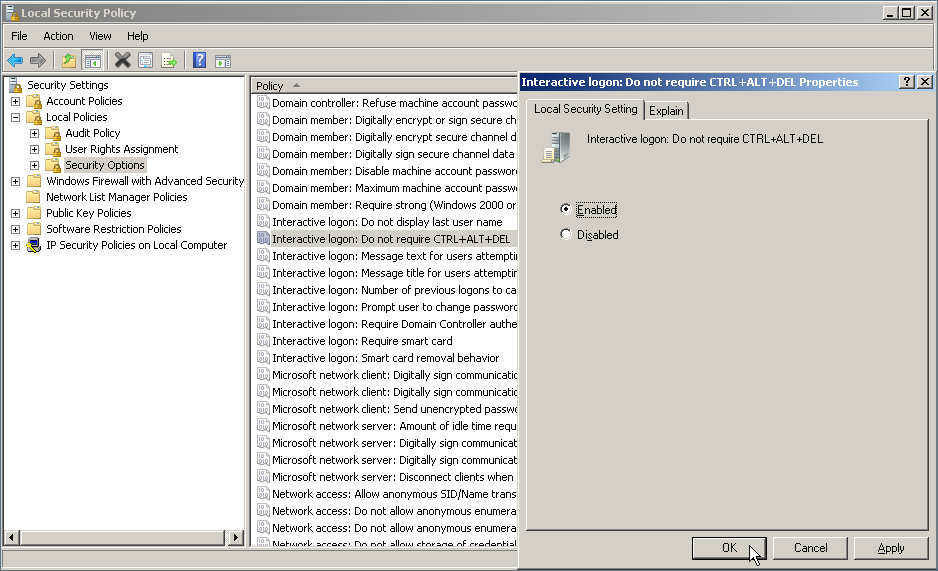
\includegraphics[scale=0.5]{images/grab0025}
 \caption{Local Security Policy.}
\label{fig:grab0025}
\end{figure}

\section{\itshape (completare)}
Implementare anche altri punti, così come evidenziato anche dal riferimento
bibliografico [4]

\section {Bibliografia}
1 Microsoft, TechNet (2009), Installazione di Windows Server 2008, http:
//technet.microsoft.com/it-it/library/cc755116(v=ws.10) \\
2 Microsoft, Download Center (2009), Windows Server 2008 Enterprise, http:
//www.microsoft.com/en-us/download/details.aspx?id=8371 \\
3 Microsoft, Supporto Tecnico (2008), Estensione del periodo di valutazione di
Windows Server 2008, http://support.microsoft.com/kb/948472 \\
4 feedback@win2008workstation.com (2012), Convert your Windows Server
2008 to a Workstation!, http://www.win2008workstation.com/
\end{document}

%\part{ITALIANO}
%\input{italiano-dante}
%\input{italiano-leopardi}

%\part{GESTIONE DEI SISTEMI}
%\input{gestione-nas.tex}

%\part{SICUREZZA INFORMATICA}
%\input{sicurezza-gpg.tex}
%\input{sicurezza-vpn.tex}



\end{document}

